\documentclass[11pt]{beamer}

\usepackage[utf8]{inputenc}
\usepackage[T1]{fontenc}
\usepackage{palatino}

% \useoutertheme{noslidenum}

\usepackage{polski}
\usepackage{subfig}
\usepackage{tikz}
\usepackage{amsmath}

\usetheme{Boadilla}

\title[Seminarium dyplomowe]{%
	Seminarium dyplomowe
}

\author[Maksymilian Skibiński]{Maksymilian Skibiński}

\date{23 maja 2022 r.}

\graphicspath{ {./img/} {./imgs_prev/} }

\captionsetup[subfigure]{labelformat = empty}

%\mode<presentation>
%{
%	\setbeamercovered{transparent}
%	% or whatever (possibly just delete it)
%}

\makeatletter
\setbeamertemplate{footline}
{
  \leavevmode%
  \hbox{%
  \begin{beamercolorbox}[wd=.333333\paperwidth,ht=2.25ex,dp=1ex,center]{author in head/foot}%
    \usebeamerfont{author in head/foot}\insertshortauthor~~\beamer@ifempty{\insertshortinstitute}{}{}
  \end{beamercolorbox}%
  \begin{beamercolorbox}[wd=.333333\paperwidth,ht=2.25ex,dp=1ex,center]{title in head/foot}%
    \usebeamerfont{title in head/foot}\insertshorttitle
  \end{beamercolorbox}%
  \begin{beamercolorbox}[wd=.333333\paperwidth,ht=2.25ex,dp=1ex,center]{date in head/foot}%
    \usebeamerfont{date in head/foot}\insertshortdate{}\hspace*{2em}
%    \insertframenumber{} / \inserttotalframenumber\hspace*{2ex} % DELETED
  \end{beamercolorbox}}%
  \vskip0pt%
}
\makeatother



\begin{document}

\frame{\titlepage}


\begin{frame}{Praca magisterska}

\textbf{Tytuł}:
\begin{center}%
Synteza oraz analiza dyskretnego układu sterowania wykorzystującego modulację PWM
\end{center}

\vspace{0.5cm}

\textbf{Promotor}: dr inż. Rafał Grygiel

\end{frame}


\begin{frame}{PWM -- Pulse Width Modulation}{Sposób kodowania informacji}

\begin{figure}[htbp!]
	\centering
	
	\subfloat[]{%
		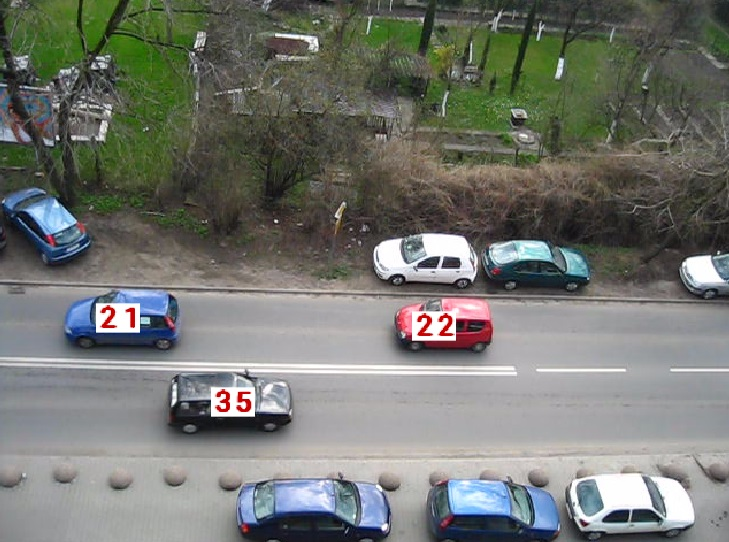
\includegraphics[width = 0.45 \linewidth]{img1}%
	}%
	\hfill%
	\subfloat[]{%
		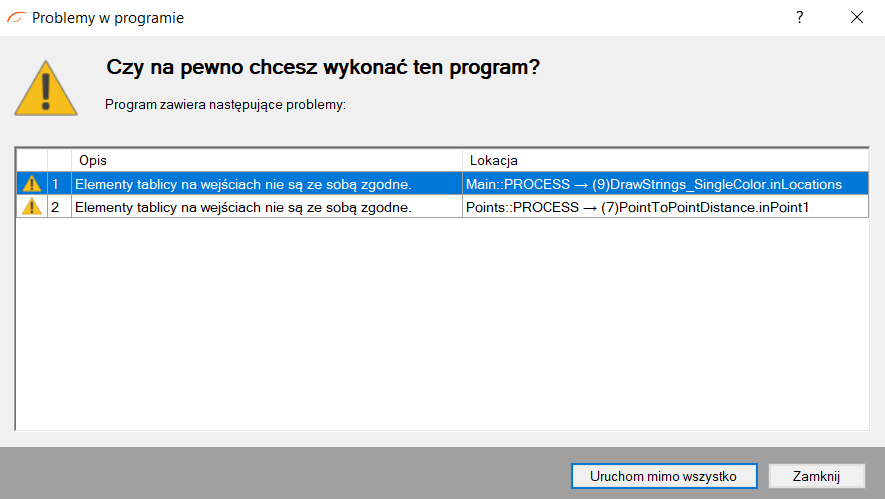
\includegraphics[width = 0.45 \linewidth]{img2}%
	}%
\end{figure}

\end{frame}


\begin{frame}{PWM -- Pulse Width Modulation}{Wypełnienie sygnału (\emph{duty cycle})}

\begin{figure}[htbp!]
	\centering
	\includegraphics[width = 0.6 \linewidth]{dt}
\end{figure}

Wartość średnia: $ \quad
\bar{y} = D \cdot y_{max} + (1 - D) \cdot y_{min}
$

\end{frame}


\begin{frame}{PWM -- Pulse Width Modulation}{Wariant trójpoziomowy}

\begin{figure}[htbp!]
	\centering
	\includegraphics[width = 0.5 \linewidth]{three}
\end{figure}

\end{frame}


\begin{frame}{PWM -- Pulse Width Modulation}{Sposób otrzymywania sygnału PWM}

\begin{figure}[htbp!]
	\centering
	\includegraphics[width = 0.6 \linewidth]{creat}
\end{figure}

\end{frame}


\begin{frame}{PWM -- Pulse Width Modulation}{Warianty sygnału piłokształtnego}

\begin{figure}[htbp!]
	\centering
	\includegraphics[width = 0.6 \linewidth]{car}
\end{figure}

\end{frame}


\begin{frame}{PWM -- Pulse Width Modulation}{Położenie impulsów}

\begin{figure}[htbp!]
	\centering
	\includegraphics[width = 0.6 \linewidth]{edge}
\end{figure}

\end{frame}


\begin{frame}{PWM -- Pulse Width Modulation}
	{Inne sposoby otrzymywania sygnału PWM -- Modulacja Delta}

\begin{figure}[htbp!]
	\centering
	\includegraphics[width = 0.65 \linewidth]{delta_v3}
\end{figure}

\end{frame}


\begin{frame}{PWM -- Pulse Width Modulation}
	{Inne sposoby otrzymywania sygnału PWM -- Modulacja Sigma-Delta}

\begin{figure}[htbp!]
	\centering
	\includegraphics[width = 0.6 \linewidth]{sigma_delta_v3}
\end{figure}

\end{frame}


\begin{frame}{UPS -- Uninterruptible Power Supply}

Układy UPS dostarczają zasilanie, gdy główne źródło nie może (np. z~powodu awarii).
Wykorzystują przetworniki mocy DC/AC (falowniki), które zaś korzystają z modulacji PWM.

\end{frame}


\begin{frame}{UPS -- Uninterruptible Power Supply}{Falownik}

\begin{figure}[htbp!]
	\centering
	\includegraphics[width = 0.85 \linewidth]{pwm_inverter}
\end{figure}

\end{frame}


\begin{frame}{UPS -- Uninterruptible Power Supply}{Falownik -- napięcia}

\begin{figure}[htbp!]
	\centering
	\includegraphics[width = \linewidth]{inv}
\end{figure}

\end{frame}


\begin{frame}{UPS -- Uninterruptible Power Supply}{Falownik w Simulinku (pakiet SimScape)}

\begin{figure}[htbp!]
	\centering
	\includegraphics[width = 0.8 \linewidth]{sim_pwm}
\end{figure}

\end{frame}


\begin{frame}{Projekt dyskretnego układu regulacji}

Projektowanie układu regulacji zostaje przeprowadzone w~oparciu o~metodę ciągłego
przybliżania układu dyskretnego w czasie.\\[10pt]

Kroki:
\begin{enumerate}
\item Układ wykorzystujący modulację PWM.
\item Układ wykorzystujący modulację PAM.
\item Układ quasi-ciągły.
\end{enumerate}

\end{frame}


\begin{frame}{Projekt dyskretnego układu regulacji}{Modulacja PWM, a PAM}

\begin{figure}[htbp!]
	\centering
	
	\subfloat[Porównanie modulacji]{%
		\includegraphics[width = 0.43 \linewidth]{pam_pwm_1}%
	}%
	\hfill%
	\subfloat[Zbliżenie na jeden impuls]{%
		\includegraphics[width = 0.43 \linewidth]{pam_pwm_2}%
	}%
\end{figure}

\end{frame}


\begin{frame}{Projekt dyskretnego układu regulacji}{Modulacja PWM, a PAM -- eksperyment}

Obiekt:
\[
K(s) = \frac{1}{1 + s}
\]

pobudzamy sygnałem sinusoidalnym.

\begin{figure}[htbp!]
	\centering
	\includegraphics[width = 0.4 \linewidth]{u}
\end{figure}

\end{frame}


\begin{frame}{Projekt dyskretnego układu regulacji}
	{Modulacja PWM, a PAM --  częstotliwość pracy modulatorów}

Niska częstotliwość pracy modulatorów -- źle.

\begin{figure}[htbp!]
	\centering
	
	\subfloat[]{%
		\includegraphics[width = 0.45 \linewidth]{uu_h1e_2}%
	}%
	\hfill%
	\subfloat[]{%
		\includegraphics[width = 0.45 \linewidth]{yy_h1e_2}%
	}%
\end{figure}

\end{frame}


\begin{frame}{Projekt dyskretnego układu regulacji}
	{Modulacja PWM, a PAM --  częstotliwość pracy modulatorów}

Wyższa częstotliwość pracy modulatorów -- lepiej.

\begin{figure}[htbp!]
	\centering
	
	\subfloat[]{%
		\includegraphics[width = 0.45 \linewidth]{uu_h1e_3}%
	}%
	\hfill%
	\subfloat[]{%
		\includegraphics[width = 0.45 \linewidth]{yy_h1e_3}%
	}%
\end{figure}

\end{frame}


\begin{frame}{Projekt dyskretnego układu regulacji}
	{Modulacja PWM, a PAM --  częstotliwość pracy modulatorów}

Jeszcze wyższa częstotliwość pracy modulatorów -- jeszcze lepiej.

\begin{figure}[htbp!]
	\centering
	
	\subfloat[]{%
		\includegraphics[width = 0.45 \linewidth]{uu_h1e_4}%
	}%
	\hfill%
	\subfloat[]{%
		\includegraphics[width = 0.45 \linewidth]{yy_h1e_4}%
	}%
\end{figure}

\end{frame}


\begin{frame}{Projekt dyskretnego układu regulacji}
	{Modulacja PWM, a PAM --  częstotliwość pracy modulatorów}

Jeszcze wyższa częstotliwość pracy modulatorów -- jeszcze jeszcze lepiej.

\begin{figure}[htbp!]
	\centering
	
	\subfloat[]{%
		\includegraphics[width = 0.45 \linewidth]{uu_h1e_5}%
	}%
	\hfill%
	\subfloat[]{%
		\includegraphics[width = 0.45 \linewidth]{yy_h1e_5}%
	}%
\end{figure}

\end{frame}


\begin{frame}{Projekt dyskretnego układu regulacji}{Modulacja PWM, a PAM -- różnice}

\begin{figure}[htbp!]
	\centering
	
	\subfloat[]{%
		\includegraphics[width = 0.45 \linewidth]{yyy1}%
	}%
	\hfill%
	\subfloat[]{%
		\includegraphics[width = 0.45 \linewidth]{yyy2}%
	}%
\end{figure}

\end{frame}



\begin{frame}{Projekt dyskretnego układu regulacji}{Aproksymacja układem z PAM}

\begin{figure}[htbp!]
	\centering
	\includegraphics[width = 0.8 \linewidth]{sim_pam}
\end{figure}

\end{frame}


\begin{frame}{Projekt dyskretnego układu regulacji}{Aproksymacja quasi-ciągła}

System sterowania (\emph{Control Unit}) jest opisany poprzez bloki:
\begin{itemize}
\item transmitancja dyskretna regulatora $H_c(z)$,
\item jednokrokowe opóźnienie $z^{-1}$,
\item wzmocnienie $k_{PWM}$.
\end{itemize}

\vspace{0.5cm}

By ,,uciąglić'' ten układ musimy go opisać przy pomocy:
\[
L(s) =
	\left( 1 - s \frac{h}{2} \right)
	\frac{\left( 1 - s \frac{h}{2} \right)}{\left( 1 + s \frac{h}{2} \right)}
	K(s)
\]

\vspace{0.5cm}

%Przejście z operatora $z$ na operator $s$:
%\[
%z^{-1} = \frac{\left( 1 - s \frac{h}{2} \right)}{\left( 1 + s \frac{h}{2} \right)}
%\]

Przejście z operatora $z$ na operator $s$:$ \qquad
z^{-1} = \frac{\left( 1 - s \frac{h}{2} \right)}{\left( 1 + s \frac{h}{2} \right)}
$

\end{frame}


\begin{frame}{Projekt dyskretnego układu regulacji}{Aproksymacja quasi-ciągła}

\begin{figure}[htbp!]
	\centering
	\includegraphics[width = 0.8 \linewidth]{sim_qct}
\end{figure}

\end{frame}


\begin{frame}{Projekt dyskretnego układu regulacji}{Aproksymacja quasi-ciągła -- schemat blokowy}

\begin{figure}[htbp!]
	\centering
	\includegraphics[width = 0.8 \linewidth]{schemat}
\end{figure}

\vspace{0.5cm}

Transmitancje:
\begin{itemize}
\item $C(s)$ -- regulator,
\item $K(s)$ -- obiekt (filtr RLC, obciążenie).
\end{itemize}

\end{frame}


\begin{frame}{Cele pracy}

\begin{itemize}
\item Porównanie układów regulacji PAM, PWM, QCR.
\item Zbadanie wpływu różnych schematów modulatora PWM na jakość regulacji.
\item Porównanie wyników z wynikami dla innego obiektu, o innej dynamice np. zbiorniki.
\end{itemize}

\end{frame}



\begin{frame}
\begin{center}
\LARGE Dziękuję za uwagę
\end{center}
\end{frame}

\end{document}